\chapter{Skupovi podataka}

Moderni informacijski sustavi stvaraju goleme količine podataka. Društvene mreže poput Facebooka, Twittera ili YouTubea imaju stotine milijuna korisnika. Društvene mreže rastu linearnom stopom te se broj korisnika u posljednjih 10 godina utrostručio što se može vidjeti i na slici \ref{fig:users}. Rastom broja korisnika raste količina informacija koja se pohranjuje te količina sadržaja i interakcija koje korisnici stvaraju. Podatke se može iskoristiti kako bi se poboljšali procesi koji se prate, pronašla područja u kojima postoji prostor za napredak, napravio iskorak u poslovanju gdje se sustav primjenjuje ili unaprijedilo korisničko iskustvo. Podaci se definiraju kao skupovi vrijednosti koji opisuju objekte u nekom procesu. Prate se kako bi se apstraktan proces iz ideje pretvorio u konkretne činjenice. Mogu se mjeriti, obrađivati i analizirati te vizualizirati kroz grafove, tablice i slike iz čega se dalje mogu izvoditi određeni zaključci. 


Algoritme koji se razvijaju da bi u podacima pronalazili korisne informacije potrebno je evaluirati te ocijeniti kako se ponašaju na kojem skupu podataka i pronaći situacije u kojima pokazuju najbolje performanse. Podaci prikupljeni iz stvarnih sustava najbolje opisuju praćene procese te je se najbolji zaključci mogu donijeti koristeći upravo njih.

\begin{figure}
	\makebox[\textwidth][c]{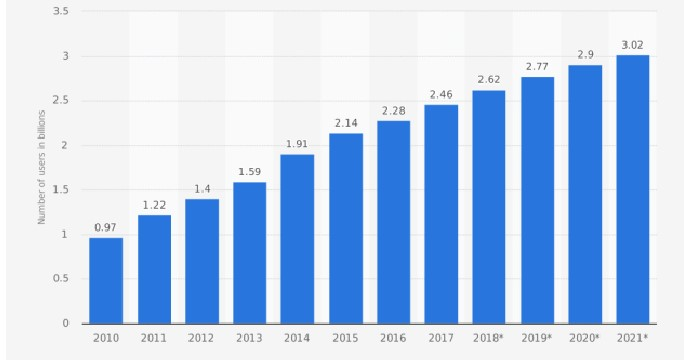
\includegraphics[width=0.8\textwidth]{images/users.jpg}}
	\caption{Kretanje broja korisnika na društvenim mrežama od 2010. do 2021. godine. Izvor \cite{usersInWorld}.}
	\label{fig:users}
\end{figure}

Nakon problema i greški tijekom prikupljanja i praćenja osobnih podataka te loše sigurnosti i slučajeva krađe podataka, 2018. godine uvedena je uredba o općoj zaštiti podataka, poznata pod kraticom GDPR. Uredbom se kontrolira pohrana, prijenos i obrada osobnih podataka u Europskoj Uniji te su navedeni procesi znatno postroženi. Nakon Europske Unije slične odredbe primijenile su i neke američke savezne države te neke Azijske države čime odredba počinje vrijediti u gotovo svim razvijenijim dijelovima svijeta. Time je područje analiza društvenih mreža značajno pogođeno jer je postalo mnogo teže dobiti podatke o stvarnim korisnicima. Od tada značajnu ulogu počinju imati algoritmi za generiranje mreža koje imaju karakteristike društvenih zajednica. Algoritmi u početnom koraku dobivaju određene podatke o veličini i svojstvima željene mreže te generiraju takav primjer. U nastavku poglavlja opisat će se Watts-Strogatz model koji generira umjetne skupove podataka te stvarni skupovi podataka pomoću kojih će se algoritmi navedeni u radu testirati.



\section{Watts - Strogatz model}

Watts-Strogatz model predstavljen je u radu \cite{watts1998collective} 1998. godine. Autori su pokušali stvoriti algoritam koji će stvoriti umjetnu mrežu, koja će imati svojstva small-world mreža koje se mogu pronaći u primjenama u biološkim, tehnološkim i društvenim sustavima. Mreže takvih sustava nalaze se između dva ekstrema, slučajne mreže i pravilne rešetkaste mreže. Kako bi se generirala mreža koja je između ta dva slučaja može se iskoristiti proces slučajnog prespajanja bridova mreže. 

Proces započinje od pravilnog grafa prstenastog oblika sa $n$ vrhova i $k$ bridova po svakom vrhu te se svaki vrh prespaja s vjerojatnosti $p$. Vjerojatnost pruža mogućnost podešavanja oblika željenog grafa između regularnog za $p = 0$ i slučajnog za $p = 1$. Strukturna svojstva generiranog grafa mjere se pomoću karakteristične duljine puta, $L$ i koeficijenta grupiranja $C$. $L$ najčešće mjeri prosječnu duljinu puta u grafu i smatra se globalnim svojstvom grafa dok $C$ mjeri koliko su susjedne veze jake te se smatra lokalnim svojstvom. Za graf kada $p \rightarrow 1$ pokazuje se da normalizirane vrijednosti $L$ i $C$ teže prema 1 , dok kada $p \rightarrow 0$ $L$ i $C$ teže prema 0 što bi moglo značiti da je velika vrijednost $C$ povezana s velikim $L$, a mala vrijednost $C$ sa malom vrijednosti $L$. No graf na slici \ref{fig:C&L} pokazuje kako se vrijednosti $L$ i $C$ mijenjaju u ovisnosti o vjerojatnosti $p$ u odnosu na broj čvorova grafa. Vidljivo je kako postoji interval u kojem je $L$ malen gotovo kao $L_{random}$ dok je $C >> C_{random}$. Takva svojstva small-world mreže moguća su zbog neposrednog pada karakteristične duljine puta $L$ uvođenjem tek nekoliko slučajnih bridova. Efekt je visoko nelinearan te se za male vrijednosti $p$ brzo smanjuje udaljenost između vrhova, ali i zajednica. Za koeficijent grupiranja prespajanje ima tek linearan utjecaj te se koeficijent gotovo ne mijenja. 

\begin{figure}
	\makebox[\textwidth][c]{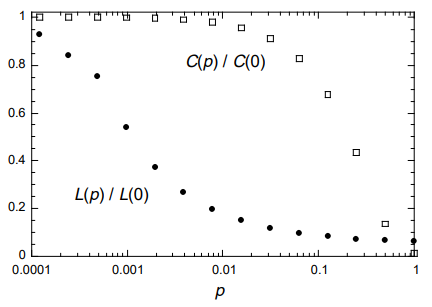
\includegraphics[width=0.7\textwidth]{images/C&L.png}}
	\caption{Karakteristična duljina puta $L$ i koeficijent grupiranja $C$ u grafovima s prespajanjem bridova u odnosu na normalizirane vrijednosti $L(0)$ i $C(0)$ za početni regularni graf. Izvor \cite{watts1998collective}.}
	\label{fig:C&L}
\end{figure}

U radu\cite{watts1998collective} ideja je provjerena na mnogo različitih početnih oblika mreža iz čega su nastali i podaci za graf \ref{fig:C&L}. Jedini uvjet je da bridovi koji se prespajaju moraju uglavnom povezivati vrhove za koje bi udaljenost bila mnogo veća nego u slučajnom grafu. Karakteristična duljina puta, $L(p)$ je definirana kao prosječna najkraća udaljenost između svih parova vrhova grafa. $C(p)$, koeficijent grupiranja, definiran je tako da ako čvor $v$ ima $k_{v}$ susjeda, onda među susjedima može postojati najviše $\frac{k_{v}(k_{v} - 1)}{2}$ bridova. Tada se $C_{v}$ definira kao omjer ostvarenih bridova među susjedima i ukupnog mogućeg broja bridova. Konačno $C$ se računa kao srednja vrijednost $C_{v}$ za svih $v$ vrhova grafa. U društvenim mrežama navedene mjere imaju smisleno značenje. $L$ je prosječan broj prijateljstava u lancu koji povezuje bilo koja dva člana zajednice. $C$ predstavlja koliko su prijatelji nekog člana zajednice povezani. Podaci prikazani u grafu \ref{fig:C&L} su uprosječeni rezultati 20 realizacija procesa slučajnog prespajanja vrhova grafa. Grafovi su imali po 1000 vrhova i prosječan stupanj vrha 10 po vrhu. Na horizontalnoj skali upotrijebljena je logaritamska skala kako bi se uspješno prikazao velik pad  $L$, dok $C$ ostaje konstantan kroz gotovo cijeli isječak koji graf prikazuje te ukazuje na činjenicu da je prelazak iz regularnog grafa prema small-world grafu gotovo neprimjetan na lokalnoj razini.


Algoritam generiranja modela grafa društvene zajednice sa small-world svojstvima odvija se kroz dva koraka. Algoritam prima tri parametra: $N$ predstavlja broj vrhova grafa, $k$ je srednja vrijednost stupnja pojedinog čvora i najčešće se odabire kao neki cijeli paran broj te $p$ što je parametar slučajnosti prespajanja promatranog brida grafa. Na konkretne parametre postoje određeni uvjeti. Vjerojatnost $p$ mora biti u granicama $0 \leq p \leq 1$. Parametri $N$ i $K$ moraju biti u sljedećem odnosu: $N >> K >> \log N >> 1$. Uvjetom $ K >> \log N$ garantira se da će generirani graf biti povezan \cite{Bollobas2001}. Algoritam konstruira neusmjereni graf sa $N$ čvorova i $\frac{NK}{2}$ bridova na sljedeći način:

\begin{enumerate}
	\item Konstruira se neusmjeren, regularan graf sa $N$ čvorova povezan sa $K$ susjeda, $\frac{K}{2}$ sa svake strane.
	\item Za svaki vrh promatra se svaki brid kojim je spojen s $\frac{K}{2}$ desnih susjeda i prespaja se s vjerojatnošću $p$. Prespajanje se obavlja tako da se brid spoji sa nekim od preostalih $v$ vrhova, različitih od trenutno promatranog i onoga s kojim ga je brid u tom trenutku povezivao, te između promatranog i odabranog vrha već ne postoji brid.
\end{enumerate}



\section{Podaci iz stvarnih društvenih mreža} \label{real_data}

Za usporedbu algoritama otkrivanja zajednica u društvenim mreža na primjerima konkretnih društvenih mreža koristit će se kolekcije podataka iz Stanford Large Network Dataset Collection \cite{snapnets}. Kolekcija se koristi u svrhu istraživanja područja o analizi društvenih i informacijskih mreža na sveučilištu Stanford. Glavni zadatak je testirati rad algoritama na stvarnim podacima gdje mogu imati korisnu primjenu. Koristit će se podaci sa društvene mreže Facebook, streaming platforme Twitch, glazbenog servisa Deezer i azijske društvene mreže LastFM. Zbog opisanih problema oko privatnosti podataka i uvođenja GDPR zakona podacima je potrebno oprezno upravljati. Stvarni podaci o korisnicima su zamijenjeni tako da se, na primjer, stvarni identifikator korisnika zamijeni surogatnim. Izmjene ne smiju utjecati na strukturalne podatke o mreži i interakcijama članova već štite privatnost korisnika.

Koristit će se podaci iz navedenih društvenih mreža sa sljedećim svojstvima:
\begin{enumerate}
	\item Facebook, 4039 vrhova i 88 234 bridova - facebook1
	\item LastFM Azija, 7624 vrhova i 27 806 bridova - LastFM
	\item Facebook, 22 470 vrhova i 171 002 bridova - facebbok
	\item Twitch, 34 118 vrhova i 429 113 bridova - twitch
	\item Deezer, 143 884 vrhova i 846 915 bridova - deezer
\end{enumerate}
Pored svojstava pojedine mreže nalaze se oznake za svaki skup podataka koje se koriste u grafovima gdje se uspoređuju rezultati algoritama.